\chapter{Largest Concatenation-Component in Regular Expressions}

\begin{center}
  April 23, 2026
  \vspace{0.5cm}
\end{center}

Hyperscan implements algorithms to decompose regexes into literals and FA in its Rose engine. There may be a relation between how well a regex can be decomposed and the size of its largest concatenation-component.

\section{Recurrences}

Let $\A$ be a finite alphabet and $\T$ be the set of all regexes excluding $\epsilon$ over $\A$. The size function $|\cdot|$ is the number of nodes.

\begin{definition}[BST-like distribution for regexes]
  We define $p:\T \to [0,1]$ as follows.
  \begin{enumerate}
    \item $\sum\limits_{c\in\A}p(c) = 1$,
    \item $p\left(\vcenter{\hbox{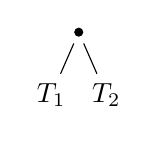
\begin{tikzpicture}[level distance=8mm, sibling distance=7mm, edge from parent/.style={draw, shorten <=1mm}]
                  \node[circle, draw, fill=black, minimum size=1mm, inner sep=0pt] {}
                  child { node {$T_1$} }
                  child { node {$T_2$} };
                \end{tikzpicture}}}\right) = \dfrac{u}{n-2} p(T_1)p(T_2)$, where $|T_1| + |T_2| = n-1$.
    \item $p\left(\vcenter{\hbox{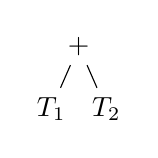
\begin{tikzpicture}[level distance=8mm, sibling distance=7mm]
                  \node{$+$}
                  child { node {$T_1$} }
                  child { node {$T_2$} };
                \end{tikzpicture}}}\right) = \dfrac{v}{n-2} p(T_1)p(T_2)$, where $|T_1| + |T_2| = n-1$.
    \item $p\left(\vcenter{\hbox{\begin{tikzpicture}[level distance=8mm, sibling distance=7mm]
                  \node{$*$}
                  child { node {$T$} };
                \end{tikzpicture}}}\right) = (1-u-v) p(T)$.
  \end{enumerate}
\end{definition}

We want to compute the expected size of the largest all-concatenation component in a regex over all of equivalent forms of its parse tree. The reason is as follows. Take the regex
$$(abc + d)(xy+z) = abcxy + abcxz + dxy + dz.$$
We expect the largest concatenation-component to be in $abcxy$ instead of $abc$ because the former is extracted by Hyperscan. Therefore, a subtree may \textit{yield} its concatenation-component to its parent if the parent is a concatenation node.

Recall the construction
$$\T = \sum_{c \in \A} c + \vcenter{\hbox{\begin{tikzpicture}[level distance=8mm, sibling distance=7mm]
        \node{$*$}
        child { node {$\T$} };
      \end{tikzpicture}}} + \vcenter{\hbox{\begin{tikzpicture}[level distance=8mm, sibling distance=7mm, edge from parent/.style={draw, shorten <=1mm}]
        \node[circle, draw, fill=black, minimum size=1mm, inner sep=0pt] {}
        child { node {$\T$} }
        child { node {$\T$} };
      \end{tikzpicture}}} + \vcenter{\hbox{\begin{tikzpicture}[level distance=8mm, sibling distance=7mm]
        \node{$+$}
        child { node {$\T$} }
        child { node {$\T$} };
      \end{tikzpicture}}}.$$
Define the random variables
\begin{enumerate}
  \item $M_n$: the largest concatenation-component that is not inside a Kleene star of a regex of size $n$ \textit{itself},
  \item $Y_n$: the largest concatenation-component that is not inside a Kleene star of a regex of size $n$ that it \textit{yields} to its parent.
\end{enumerate}

We have the following recurrences
\begin{align}
  Y_{n+2}
   & =\begin{cases}
        Y_{U_n}^{(1)} + Y_{n+1-U_n}^{(2)} + 1  & \text{prob. } u,    \\
        \max(Y_{U_n}^{(1)}, Y_{n+1-U_n}^{(2)}) & \text{prob. } v,    \\
        0                                      & \text{prob. } 1-u-v
      \end{cases}                                                                      & Y_1=Y_2=0.                         \label{eq:yield}                           \\
  M_{n+2}
   & = \begin{cases}
         \max(Y_{U_n}^{(1)} + Y_{n+1-U_n}^{(2)} + 1, M_{U_n}^{(1)}, M_{n+1-U_n}^{(2)}) & \text{prob. } u,    \\
         \max(M_{U_n}^{(1)}, M_{n+1-U_n}^{(2)})                                        & \text{prob. } v     \\
         0                                                                             & \text{prob. } 1-u-v
       \end{cases} & M_1=M_2=0.
\end{align}

We have used $Y_n^{(1)}, Y_n^{(2)}, M_n^{(1)}, M_n^{(2)}$ as independent copies of $Y_n$ and $M_n$ respectively, and $U_n$ as a uniform random variable over $\{1, 2, \ldots, n\}$ independent of all $Y_n^{(i)}$ and $M_n^{(i)}$.

\section{The yield recurrence}

\subsection{Asymptotic of the Expectation}

Consider the case $2u+v>1$. By the bounds,  there exists
$$\alpha = \inf\left\{\beta: \dfrac{Y_n}{n^\beta} \xlongrightarrow{d} 0\right\}.$$

We know that $\alpha \in (2u+v-1, 2(u+v)-1]$. We want to see if indeed $y_n \sim C n^\alpha$ for some $C>0$.

We try the contraction method \cite{ludgercontraction,neininger2004general, drmota2009random}. Let us mention some conventions. For a random variable $X$, denote by $\L(X)$ its distribution. Let $(\M, d)$ be a metric space where $\M$ is a set of probability distributions of our random variables and the metric $d$ is such that $d(\L(X),\L(Y))=0$ implies $X \stackrel{d}{=} Y$. The idea is as follows

\begin{enumerate}
  \item Guess a normalization $X_n$ of $Y_n$ that converges in distribution.
  \item Plug $X_n$ into the recurrence. Assume that $X_n$ converges, show that the limit equation has a unique solution $X^*$. This is done by proving that the operator $T$ defined by the right-hand side of the limit equation is a contraction.
  \item Prove that indeed $d(\L(X_n), \L(X^*)) \to 0$.
\end{enumerate}

The method is use to obtain more information about the limit distribution of $X_n$ rather than just its expectation. For example, the following is the recurrence for the number of comparisons in Quicksort where the first element is chosen as the pivot \cite{drmota2009random}
$$Y_{n} = Y_{U_n}^{(1)} + Y_{n-1-U_n}^{(2)} + n-1.$$
One can find the asymptotic of $\EE[Y_n]$ by taking expectation on both sides. The contraction is then used to show that $X_n = \dfrac{Y_n - \EE[Y_n]}{n}\to X^*$, where the denominator $n$ is the ``guessed'' variance.

Our case is weaker. The normalization is $X_n = Y_n / n^{\alpha}$ such that $X_n\xlongrightarrow{d}X^*$. Plugging into the recurrence (\ref{eq:yield_indicator}), we have
\begin{align*}
  (n+2)^\alpha X_{n+2} \stackrel{d}{=} \,\,
   & I\left(U_n^\alpha X_{U_n}^{(1)} + (n+1-U_n)^\alpha X_{n+1-U_n}^{(2)} + 1\right)  \\
   & + J\max\left(U_n^\alpha X_{U_n}^{(1)}, (n+1-U_n)^\alpha X_{n+1-U_n}^{(2)}\right)
\end{align*}
Equivalently,
\begin{equation}
  \begin{aligned}
    X_{n+2} \stackrel{d}{=}\,\,
     & I\left(\left(\dfrac{U_n}{n+2}\right)^\alpha X_{U_n}^{(1)} + \left(\dfrac{n+1-U_n}{n+2}\right)^\alpha X_{n+1-U_n}^{(2)} + \dfrac{1}{(n+2)^\alpha}\right) \\
     & + J\max\left(\left(\dfrac{U_n}{n+2}\right)^\alpha X_{U_n}^{(1)}, \left(\dfrac{n+1-U_n}{n+2}\right)^\alpha X_{n+1-U_n}^{(2)}\right)
  \end{aligned}
\end{equation}

\begin{proposition}
  The right-hand side of the above recurrence converges in distribution to
  \begin{equation}
    I\left(U^\alpha X^{(1)} + (1-U)^\alpha X^{(2)}\right) + J\max\left(U^\alpha X^{(1)}, (1-U)^\alpha X^{(2)}\right)
  \end{equation}
\end{proposition}

\begin{proof}
  We first show that
  $$\left(\dfrac{U_n}{n+2}\right)^\alpha X_{U_n}^{(1)} + \left(\dfrac{n+1-U_n}{n+2}\right)^\alpha X_{n+1-U_n}^{(2)} \xlongrightarrow{d} U^\alpha X^{(1)} + (1-U)^\alpha X^{(2)}.$$

  By Lemma \ref{lemma:average_uniform_convergence} and Slutsky's theorem,
  $$\dfrac{U_n}{n+2} = \dfrac{U_n}{n} \cdot \dfrac{n}{n+2} \xlongrightarrow{d} U.$$

  To apply the Continuous Mapping Theorem, we need to show that
  $$\left(\dfrac{U_n}{n+2}, X_{U_n}^{(1)}, X_{n+1-U_n}^{(2)}\right) \xlongrightarrow{d} \left(U, X^{(1)}, X^{(2)}\right).$$

  Since $U, X^{(1)}, X^{(2)}$ are independent, this is equivalent to showing that $\forall u, x_1, x_2 \in \mathbb{R}$
  $$\PP\left(U_n \le \lfloor nu \rfloor, X_{U_n}^{(1)} \le x_1, X_{n+1-U_n}^{(2)} \le x_2\right) \longrightarrow \PP(U \le u) \PP(X^{(1)} \le x_1) \PP(X^{(2)} \le x_2).$$

  Indeed,
  \begin{align*}
     & \PP\left(U_n \le \lfloor nu \rfloor, X_{U_n}^{(1)} \le x_1, X_{n+1-U_n}^{(2)} \le x_2\right)                                                                         \\
     & = \sum_{k=1}^{\lfloor nu \rfloor} \PP(U_n=k) \PP\left(X_{k}^{(1)} \le x_1, X_{n+1-k}^{(2)} \le x_2 | U_n=k\right)                                                    \\
     & =  \dfrac{1}{n}\sum_{k=1}^{\lfloor nu \rfloor} \PP\left(X_{k}^{(1)} \le x_1, X_{n+1-k}^{(2)} \le x_2\right)               & (U_n\bot (X_{k}^{(1)}, X_{n+1-k}^{(2)})) \\
     & =  \dfrac{1}{n}\sum_{k=1}^{\lfloor nu \rfloor} \PP\left(X_{k}^{(1)} \le x_1\right)\PP\left(X_{n+1-k}^{(2)} \le x_2\right) & (X_{k}^{(1)} \bot X_{n+1-k}^{(2)})       \\
  \end{align*}

  Let $F_n$ be the common CDF of $X_n^{(1)}$ and $X_n^{(2)}$, and $F$ be the CDF of $X^{(1)}$. Let $m = \lfloor nu \rfloor$. The problem becomes showing that
  $$\dfrac{1}{n}\sum_{k=1}^{m} F_k(x_1)F_{n+1-k}(x_2) \longrightarrow u F(x_1) F(x_2).$$
  Equivalently,
  $$\dfrac{m}{n}\left(\dfrac{1}{m}\sum_{k=1}^{m} \left(F_k(x_1)F_{n+1-k}(x_2)-F(x_1) F(x_2)\right)\right) \longrightarrow 0.$$

  We have
  \begin{align*}
     & \dfrac{1}{m}\sum_{k=1}^{m} \left|F_k(x_1)F_{n+1-k}(x_2)-F(x_1) F(x_2)\right|                                                                                                       \\
     & \le \dfrac{1}{m}\sum_{k=1}^{m} \left|F_k(x_1)\left(F_{n+1-k}(x_2)-F(x_2)\right)\right| + \dfrac{1}{m}\sum_{k=1}^{m} \left|F(x_2)\left(F_k(x_1)-F(x_1)\right)\right|                \\
     & \le \dfrac{1}{m}\sum_{k=1}^{m} \left|F_{n+1-k}(x_2)-F(x_2)\right| + \dfrac{1}{m}\sum_{k=1}^{m} \left|F_k(x_1)-F(x_1)\right|                                         & (|F_n|\le 1) \\
  \end{align*}
  The second term goes to zero by the fact that $F_n(x_1)\to F(x_1)$ and Cesàro Means. We can write the first term as
  \begin{align*}
    \dfrac{1}{m}\sum_{k=n-m+1}^{n} \left|F_{k}(x_2)-F(x_2)\right|.
  \end{align*}

  If $u=1$, its convergence is similar to the second term. If $u<1$, then $n-m+1 \to \infty$. By pointwise convergence,$\forall \epsilon>0, \exists N, \forall n\ge N: |F_n(x_2)-F(x_2)|<\epsilon$. Hence, for $n-m+1\ge N$,
  \begin{align*}
    \dfrac{1}{m}\sum_{k=n-m+1}^{n} \left|F_{k}(x_2)-F(x_2)\right| < \epsilon.
  \end{align*}

  Using Slutsky's theorem again, we have

  $$\left(\dfrac{n+1}{n+2}, \dfrac{U_n}{n+2}, X_{U_n}^{(1)}, X_{n+1-U_n}^{(2)}\right) \xlongrightarrow{d} \left(1, U, X^{(1)}, X^{(2)}\right).$$

  Now define the function $f:\mathbb{R}^4_+\cap \left\{(t,u,x,y): t\ge u\right\} \to \mathbb{R}$ by
  $$f(t,u,x,y) = u^\alpha x + (t-u)^\alpha y.$$
  Then $f$ is continuous. The Continuous Mapping Theorem applies. The convergence
  $$\max\left(\left(\dfrac{U_n}{n+2}\right)^\alpha X_{U_n}^{(1)}, \left(\dfrac{n+1-U_n}{n+2}\right)^\alpha X_{n+1-U_n}^{(2)}\right) \xlongrightarrow{d} \max\left(U^\alpha X^{(1)}, (1-U)^\alpha X^{(2)}\right)$$

  is similar. And finally, we define the continuous function $g(i,j,u,v) = iu+jv$ on $\RR^4$ to finish the proof.


\end{proof}
% \begin{proposition}
%   Let $T:\M\to \M$ be an operator in the space of probability distributions with finite expectation, defined by

%   $$T(\mu) = \L\left(I(U^\alpha X^{(1)} + (1-U)^\alpha X^{(2)}) + J\max(U^\alpha X^{(1)}, (1-U)^\alpha X^{(2)})\right),$$
%   where $X^{(1)}, X^{(2)} \overset{\text{iid}}{\sim} \mu$, $U$ is uniformly distributed on $[0,1]$, $I$ and $J$ are Bernoulli with expectation $u$ and $v$ respectively, such that $I+J\le 1$. The variables $U, I, J$ and $(X^{(1)}, X^{(2)})$ are mutually independent.
%   Then there exists $p\ge 2$ such that $T$ is a contraction in the $(\M_p, \ell_p)$, where the $\ell_p$ metric is defined by
%   $$\ell_p(\mu, \nu) = \inf\{\EE[|X-Y|^p]: X\sim \mu, Y\sim \nu\}.$$
% \end{proposition}

% \begin{proof}
%   Let $\mu,\nu \in \M_p$. Let $X, X^{(1)}, X^{(2)} \overset{\text{iid}}{\sim} \mu$ and $Y, Y^{(1)}, Y^{(2)} \overset{\text{iid}}{\sim} \nu$ be independent of each other. We have
%   \begin{align*}
%     \ell_p(T(\mu), T(\nu))
%      & = \EE\left[\left|I(U^\alpha X^{(1)} + (1-U)^\alpha X^{(2)}) + J\max(U^\alpha X^{(1)}, (1-U)^\alpha X^{(2)})\right.\right.                         \\
%      & \,\,\,\, \left.\left.- I(U^\alpha Y^{(1)} + (1-U)^\alpha Y^{(2)}) - J\max(U^\alpha Y^{(1)}, (1-U)^\alpha Y^{(2)})\right|\right]                   \\
%      & \le \EE\left[\left|I \left(U^\alpha X^{(1)} + (1-U)^\alpha X^{(2)} - U^\alpha Y^{(1)} - (1-U)^\alpha Y^{(2)}\right)\right|\right]                 \\
%      & \,\,\,\, + \EE\left[\left|J\left(\max(U^\alpha X^{(1)}, (1-U)^\alpha X^{(2)}) - \max(U^\alpha Y^{(1)}, (1-U)^\alpha Y^{(2)})\right)\right|\right]
%   \end{align*}

%   Consider the first term. We have
%   \begin{align*}
%              & \EE\left[\left|I \left(U^\alpha X^{(1)} + (1-U)^\alpha X^{(2)} - U^\alpha Y^{(1)} - (1-U)^\alpha Y^{(2)}\right)\right|\right]                                       \\
%     = \,\,   & \EE\left[I\left| \left(U^\alpha X^{(1)} + (1-U)^\alpha X^{(2)} - U^\alpha Y^{(1)} - (1-U)^\alpha Y^{(2)}\right)\right|\right]        & (I\ge 0)                     \\
%     =  \,\,  & u \EE\left[\left|U^\alpha \left(X^{(1)} - Y^{(1)}\right) + (1-U)^\alpha \left(X^{(2)} - Y^{(2)}\right)\right|\right]                 & \text{(independence of $I$)} \\
%     \le \,\, & u \left(\EE\left[U^\alpha \left|X^{(1)} - Y^{(1)}\right|\right] + \EE\left[(1-U)^\alpha \left|X^{(2)} - Y^{(2)}\right|\right]\right) & (U, 1-U \ge 0)               \\
%     = \,\,   & \dfrac{2u}{\alpha+1} \EE[\left|X - Y\right|].
%   \end{align*}

%   We turn to the second term. Recall that $|\max(a,b) - \max(c,d)| \le \max(|a-c|, |b-d|)$ and $\max(a,b) = \dfrac{1}{2}(a+b + |a-b|)$ for any real numbers $a,b,c,d$. We have
%   \begin{align*}
%         & \EE\left[\left|J\left(\max(U^\alpha X^{(1)}, (1-U)^\alpha X^{(2)}) - \max(U^\alpha Y^{(1)}, (1-U)^\alpha Y^{(2)})\right)\right|\right]                                                   \\
%     \le & v\EE\left[\max\left(\left|U^\alpha\left(X^{(1)} -  Y^{(1)}\right)\right| ,\left|(1-U)^\alpha \left(X^{(2)} - Y^{(2)}\right)\right|\right)\right]                                         \\
%     =   & \dfrac{v}{2} \left(\EE\left[U^\alpha\right]\EE\left[\left|X^{(1)} - Y^{(1)}\right|\right] + \EE\left[(1-U)^\alpha\right]\EE\left[\left|X^{(2)} - Y^{(2)}\right|\right]\right.            \\
%         & \left.+ \EE\left[\left|U^\alpha\left(X^{(1)} -  Y^{(1)}\right) - (1-U)^\alpha\left(X^{(2)} - Y^{(2)}\right)\right|\right]\right)                                                         \\
%     =   & \dfrac{v}{\alpha+1} \EE\left[\left|X - Y\right|\right]  + \dfrac{v}{2} \EE\left[\left|U^\alpha\left(X^{(1)} -  Y^{(1)}\right) - (1-U)^\alpha\left(X^{(2)} - Y^{(2)}\right)\right|\right] \\
%   \end{align*}

%   Combining the bounds for both terms, we get
%   $$\ell_1(T(\mu), T(\nu)) \le \dfrac{2u}{\alpha+1} \EE[|X - Y|] + J \EE[|X - Y|].$$

%   Since $\dfrac{2u}{\alpha+1} + J < 1$, the operator $T$ is a contraction in the $(\M_1, \ell_1)$ space.


% \end{proof}


